\section{Actividad 1}

\subsection*{a) Si las señales recibidas se suman en la antena receptora. ¿Cuál es el resultado de esto? Graficar. }

Las señales recibidas se expresan de la siguiente manera:

    \[
        y_1(t) = 0.9 \cdot 17 \cos(2\pi f_1 (t - \tau_1))
        \]
        \[
        y_2(t) = 0.75 \cdot 17 \cos(2\pi f_1 (t - \tau_2))
    \]

donde los retardos temporales son calculados como:

    \[
        \tau_1 = \frac{D_1}{c} = \frac{11000}{3 \times 10^8} = 36.67 \, \mu s
        \]
        \[
        \tau_2 = \frac{D_2}{c} = \frac{14500}{3 \times 10^8} = 48.33 \, \mu s
    \]

La señal resultante es la suma de la señal transmitida por un camino directo y de la señal reflejada \(y(t) = y_1(t) + y_2(t)\) 
\bigskip


\begin{figure}[H]
    \centering
        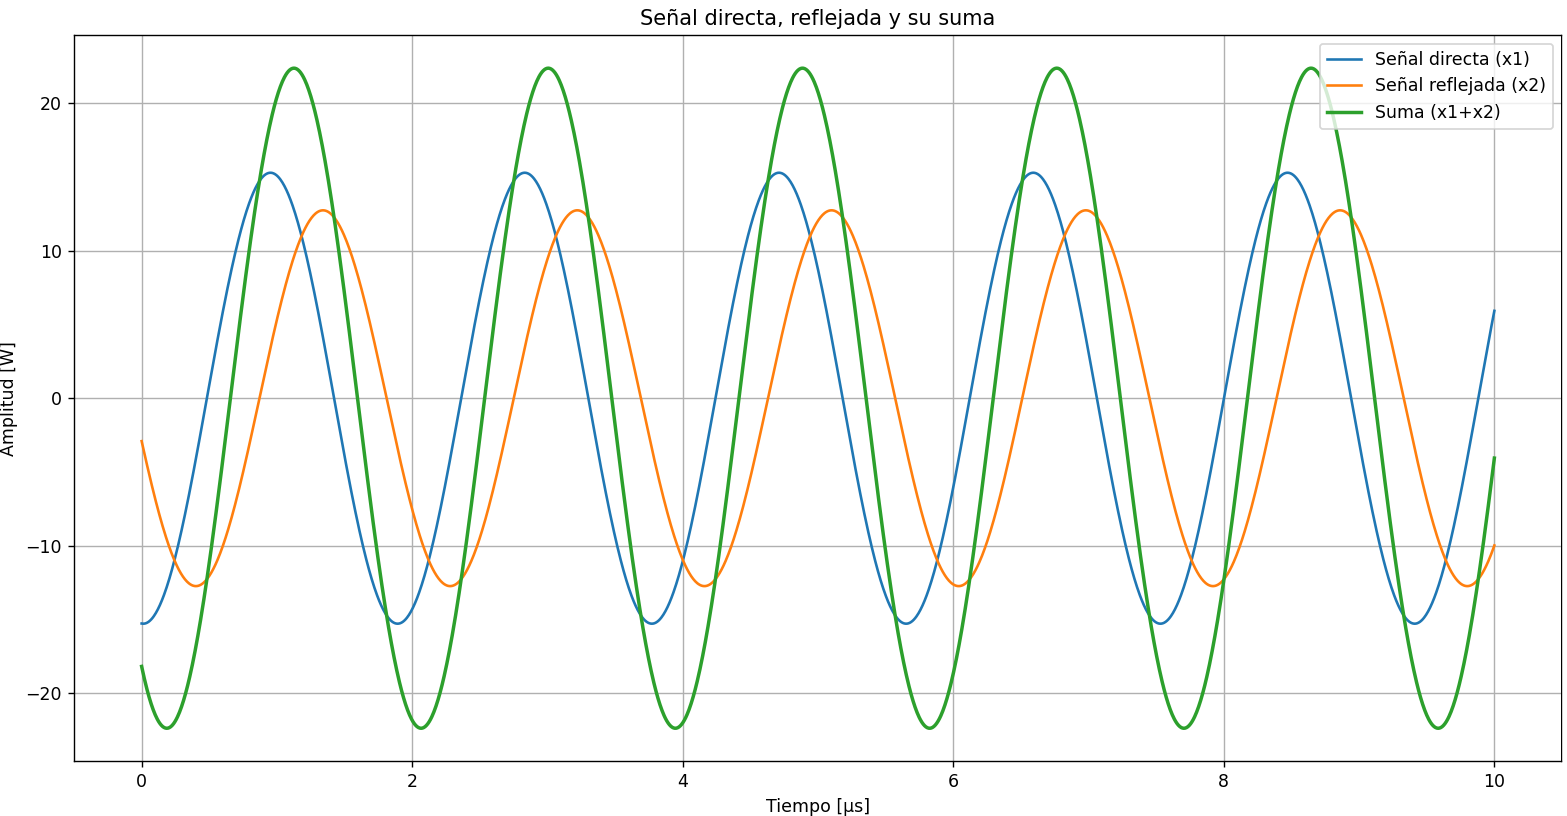
\includegraphics[width=0.8\textwidth]{imagenes/Actividad_1/grafico_532kHz.png}
        \caption{Señal resultante a 532 kHz.}
        \label{fig:532kHz}
    \end{figure}
\bigskip

En la Fig. \ref{fig:532kHz} se observa la señal cosenoidal trasmitida en su camino directo y reflejado, la suma de las dos es la que 
llega a la antena receptora. Como se observa, tienen diferente amplitud y fase debido a las atenuaciones y un retardo temporal por las 
diferentes distancias.
\bigskip

\subsection*{b) Suponer ahora que la frecuencia aumenta a 600 kHz. ¿Qué sucede? Graficar. }

Hay dos trayectorias:
    \[
         D_1 = \SI{11}{km} \qquad D_2 = \SI{14.5}{km}.  
    \]
\bigskip

La diferencia es:
    \[
        \Delta D = D_2 - D_1 = \SI{3.5}{km} = \SI{3500}{m}.
    \]
\bigskip

El retardo entre ambas:
    \[
        \Delta \tau = \frac{\Delta D}{c} = 
        \frac{3500}{3 \cdot 10^{8}}
        \approx 1.1667 \times 10^{-5}\,\text{s}.
    \]

\bigskip

La diferencia de fase entre ellas es:
    \[
        \Delta\varphi = 2\pi f \,\Delta\tau.
    \]


Las dos señales quedan en fase cuando su diferencia de fase es un múltiplo entero de \(2\pi\):
    \[
        \Delta\varphi = 2\pi n,\qquad n=0,1,2,\dots
    \]


    \[
        2\pi f \,\Delta\tau = 2\pi n \quad\Longrightarrow\quad f=\frac{n}{\Delta\tau}.
    \]
\bigskip

Para \(\Delta\tau=1.1667\times10^{-5}\,\text{s}\):
    \[
        f_n=\frac{n}{1.1667\times10^{-5}}.
    \]
\bigskip

Para \(n=7\):
    \[
        f_7=\frac{7}{1.1667\times10^{-5}}=600\,\text{kHz}.
    \]
\bigskip

A \(f=600\,\text{kHz}\) la diferencia de fase es:
    \[
        \Delta\varphi=2\pi f \,\Delta\tau=2\pi\cdot 600000\cdot1.1667\times10^{-5}
        =2\pi\cdot 7=14\pi,
    \]
que es exactamente 7 ciclos completos de diferencia. Por lo tanto, las señales quedan en fase. Por lo tanto, la señal resultante se 
observa en la Fig. \ref{fig:600kHz}.

    \begin{figure}[H]
        \centering
        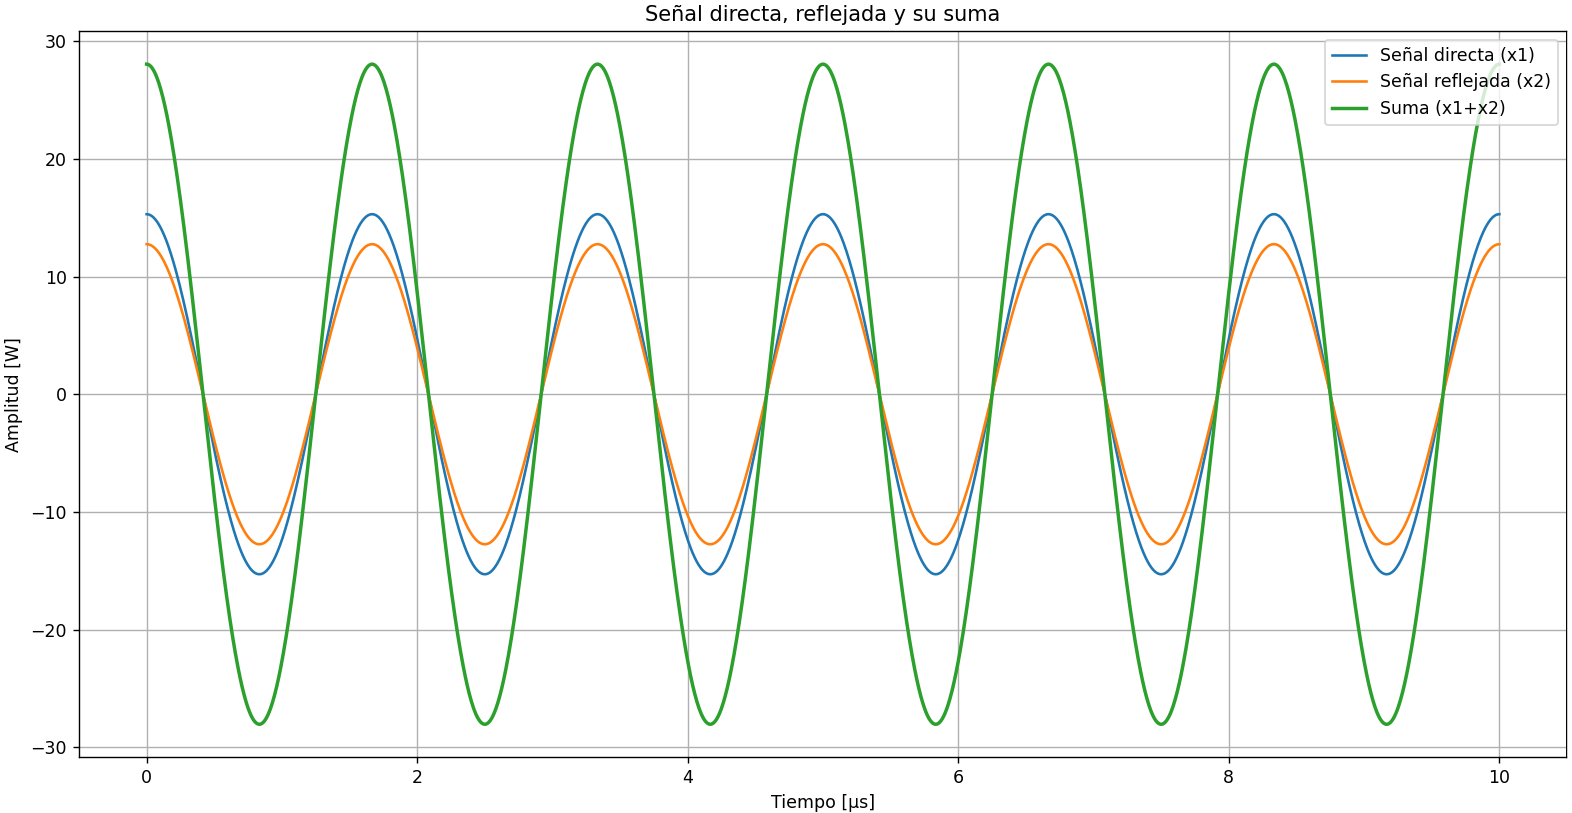
\includegraphics[width=0.8\textwidth]{imagenes/Actividad_1/grafico_600kHz.png}
        \caption{Señal resultante a 600 kHz.}
        \label{fig:600kHz}
    \end{figure}
